
\documentclass{article}

\usepackage{arxiv}
\usepackage{graphicx}

\usepackage[utf8]{inputenc} % allow utf-8 input
\usepackage[T1]{fontenc} % use 8-bit T1 fonts
\usepackage{hyperref} % hyperlinks
\usepackage{url} % simple URL typesetting
\usepackage{booktabs} % professional-quality tables
\usepackage{amsfonts} % blackboard math symbols
\usepackage{nicefrac} % compact symbols for 1/2, etc.
\usepackage{microtype} % microtypography
\usepackage{lipsum}
\usepackage{float}

\usepackage{lineno}
\linenumbers

\title{Review of current simple ultrasound hardware considerations, designs, and processing opportunities}

%% Rev2t https://gist.github.com/kelu124/ca6f58c2c5e1de3134df5a76fff4e48a



\author{
 Luc Jonveaux\thanks{Lead of the un0rick.cc project } \\
 Open-source hobbyist \\
 Milly le Meugon, FR\\
 \texttt{kelu124@gmail.com} \\
 \And
 Carla Schloh \\
 Fraunhofer MEVIS\\
 Institute for Digital Medicine\\
 Bremen, DE\\
 \texttt{ carla.schloh@yahoo.de} \\
\And
 William Meng \\
Stanford University \\
 Stanford, CA, US\\
 \texttt{ wlmeng@stanford.edu} \\
 %% examples of more authors
 \And
 Jorge Arija \\
MicroComp \\
 Bilbao, ES\\
 \texttt{ jarija@microcomp.es} \\
   \And
 Jean Rintoul \\
Mindseye Biomedical \\
 London, UK\\
 \texttt{ jean@mindseyebiomedical.com} \\
 }


\begin{document}
\maketitle

\begin{abstract}

Ultrasound is one of the most widely used imaging tools for non-destructive testing (NDT) and non-invasive medical diagnosis.
Since its beginnings in the 1970s, ultrasound imaging has been an ongoing field of research,
with innovations such as new sensors, signal processing, and hardware development. After more than fifty years, the field still presents active developments, aided by advances in electronics and digital hardware.

However, within the realm of open-source equipment, the field remains under-researched in terms of experimental hardware. An open, flexible and cost-efficient platform is still needed for many medical and testing basic applications to support the efforts of the researchers, makers and device developers, to accelerate ultrasound research and development.

The aim of this review is to identify literature that is relevant for understanding, designing and operating a simple ultrasound device, and to capture this body of knowledge and make it accessible to ultrasound system designers. It also aims at presenting current ultrasound research focus points to introduce the reader to trends of interest.

We try to capture design and use considerations from older and newer designs. We have covered both NDT and medical applications, starting with a review of the context, following on the review of existing architectures and analog buildings blocks, then on digital options available to support and complement the hardware aspects.

This body of knowledge was used for designing two relatively simple open hardware designs.



\end{abstract}


% keywords can be removed
\keywords{ultrasound \and hardware \and open-source \and frugal device \and imaging \and modular design}

% this table is to be removed before submission
%\tableofcontents

\newpage


\section{A renewed interest in ultrasound hardware}

Ultrasound has been a developing field for medical imaging and non-destructive testing and exploration (NDT/NDE) since the 1950s. Although ultrasound is today a relatively mature technology \cite{kjeken_systematic_2011}, it remains an active field of study \cite{lanza_ultrasound_2020}. 
New technologies such as Capacitive Micromachined Ultrasound Transducers (CMUTs) and Compressed Sensing (CS) \cite{kruizinga_compressive_2017, liebgott_compressive_2012}, have the potential to revolutionize ultrasound imaging and drastically improve its affordability. Ultrasound imaging has numerous advantages over other widely-used imaging modalities, such as computer tomography (CT), X-ray imaging or magnetic resonance tomography (MRI), particularly because it is deemed safe and affordable \cite{kurjak_use_1986}, and has become an important tool in medical care \cite{wang_anatomy_2020}. 

Renewed interest in ultrasound technologies also is the development of multi-modalities devices, systems that combine ultrasound with electrical, MRI, optical and tomography imaging modalities, especially in light of the recent piezoelectric organic light-emitting diodes \cite{yu_direct_2020}, or non-contact laser ultrasound \cite{zhang_full_2019}. These developments have the potential to drastically change the ultrasound hardware paradigm. It would therefore make sense to build an open, affordable and extensible platform for ultrasound research. It leverages progress in low-cost computing in order to offload functions which previously required complex and expensive hardware. From our community, we see users from college students to post-docs, on matters to non-destructive testing or medical imaging fields.

We keep an open-hardware approach for this review, as open-hardware has been shown to lower barriers to product research \cite{pandey_open_2019}, promote technology use, and  can have a disruptive effect on the ultrasound market by enabling shorter development cycles, which allows for more rapid iterations of products \cite{pearce_quantifying_2015, pearce_return_2016, moritz_economic_2019, winter_open_2019} as well as allowing users to access and repair devices, Using freely-available online documentation and support from the open source community \cite{gibney_open-hardware_2016}. 

\section{The main ultrasound imaging modes}


With the exception of Doppler imaging, ultrasound imaging is based on the "pulse-echo" principle, which relies on the dual receiver-transmitter function of a piezoelectric transducer. For the sake of the present review, we will voluntarily discard the review of Doppler-related modes, including C-Mode, spectrogram and others, which lie beyond the scope of simple imaging methods. The two main modes commonly found in ultrasound equipment are:

\textbf{\textit{A-Mode}}, or amplitude mode, is used to display the direct amplitude of echoes received as a function of time and creates one-dimensional images. We would deem M-Mode (as a A-Mode time \bold{m}otion display) an extension of the A-mode. This is the building block of B-mode imaging.

\textbf{\textit{B-Mode}}: in B-Mode ultrasound, the most common form of ultrasound imaging, a 2D image is produced. It displays the envelope of the recorded symbols, typically in grey-value representation on a 2D map where every value is assigned a different shade of grey. The higher the intensity of the echo, the brighter the reflection interface in the reconstructed image. This is the widely known sonogram used to examine babies in utero. As a reference for the next sections, the reviewed literature offers a view of a minimal B-mode imaging system, in particular thanks to \cite{kurjak_use_1986} who laid out the basic specifications for a general purpose ultrasound scanner. This basic, minimal specification set can allow designers to frame the development of their own systems, captured in precursor portable devices such as with the Sonovisor \cite{zeiss_sonovisor_1962} or later portable devices \cite{ligtvoet_real_1978}, which would have to be able to:

\begin{itemize}
\setlength\itemsep{0.01em}
\item produce B-mode images, which translates as a device having linear- and convex- type scan-heads
\item image with a frequency of 3.5 to 5MHz, for a depth of up to 18cm
\item image human tissues with at least 50dB of SNR \cite{attarzadeh_low-power_2017}, which requires at least a 9-bit ADC 
\item display a reconstructed 512 x 512 image, with a depth of 4 bits 
\item scan a viewing angle of 40 degrees or more, which indicates that 128 lines per image should be sufficient.
\item refresh the image at 5 to 10fps.
\end{itemize}



A less commonly used mode is \textbf{\textit{tomography}}. Though less common than the previously discussed uses, ultrasound can be used in tomography for imaging soft tissue \cite{zhang_design_2015, duric_detection_2007, wen_design_2019, ashfaq_new_2004,marwa_automatic_2019,gemmeke_hardware_2010}. A single transducer or array of transducers is used to measure acoustic impedance at different angles and an image is reconstructed using back-projection or related finite element techniques. The same acoustic impedance methods used in tomography have also been used to recreate images with high temporal and spatial resolution in recent research on plane wave acoustic imaging \cite{Rabut2019,Warner2013}. New computing techniques for full wave imaging have also the opened door to better imaging \cite{guasch_full-waveform_2020, rymarczyk_logistic_2019}. 



% \textbf{\textit{Overall imaging}}: although it is relatively simple and does not enable 2D imaging, A-mode enables measurements for examinations such as para-nasal sinuses, trans-skull fluid detection, sinus pathology, skeletal muscle detection in the wrist extension \cite{noauthor_wrist_nodate}, measurement of the artery lumen diameter \cite{hu_design_2011, zhang_multi-channel_2017, shomaji_early_2019}, bone porosity \cite{wahab_design_2016, fontes-pereira_monitoring_2018, grasel_characterization_2017} and ophthalmology assessments \cite{carotenuto_very_2004}.

%Ultrasound can be used for \textbf{\textit{Vascular assessments}}, to measure the diameter and the blood pulse speed traveling through the radial artery \cite{worthing_using_2016}, which then can be used to track changes in blood pressure at various points on the human body. 
%Other \textbf{\textit{body monitoring}} uses include artery stiffness measurements \cite{joseph_technical_2015, joseph_artsenstouch_2015, seo_non-invasive_2018}, monitoring bone density \cite{wahab_design_2016, fontes-pereira_monitoring_2018},tissue assessment \cite{keyes_electrical_2017}, including muscle evolution \cite{brausch_towards_2019} for example quantifying neuro-muscular disease progression \cite{zhang_design_2015}, both using A-mode and B-mode imaging. 

%\textbf{\textit{Body composition assessment}} is another application of A-mode imaging \cite{wagner_validity_2016, martins_-scan_2017}. The measurement of \textbf{\textit{bladder volumes}} is also a standard medical use \cite{kuru_feasibility_2019}. 

%Another use can be providing \textbf{\textit{biofeedback}}, as it has been shown that ultrasound imaging enables the tracking of muscle movements \cite{sikdar_novel_2014} and follow-up of biofeedback in stroke reeducation \cite{sosnowska_training_2019}. 

%Last but not least, ultrasound has also been used in \textbf{\textit{tracking body movements}}, for example, tracking obstructive sleep apnea \cite{weng_fpga-based_2015}, breathing patterns \cite{shahshahani_ultrasound_2018}, and heart muscle behavior \cite{nguyen_estimating_2019}.

%Other interesting uses include the development of \textbf{\textit{ultrasound capsules}}, typically swallowable devices, which enable endoscopy imaging using high frequency ultrasound by fitting the hardware into a 10mm diameter by 30 mm long capsule \cite{cox_ultrasound_2017, wang_development_2017}. Capsules promise further development, and their architecture can be a source of inspiration \cite{lee_towards_2014, memon_capsule_2016, lay_progress_2016, lay_-vivo_2018}. \textbf{\textit{Wearable devices}} are also gaining momentum due to the miniaturisation trend in components and sensors \cite{basak_wearable_2013}. This is also seen in \textbf{\textit{neuromodulation}} \cite{pashaei_flexible_2020} applications, where ultrasound is used both to power implants, communicate with them or between them \cite{johnson_stimdust_2018, seo_wireless_2016, santagati_design_2020}, and even to stream video \cite{kou_real-time_2020}.

%Ultrasound is also used for \textbf{\textit{nondestructive testing (NDT)}} or nondestructive examination (NDE)  \cite{duncan_real-time_1990,noauthor_integration_nodate}, for quality or integrity control of mechanical elements. \cite{fritsch_full_nodate} presents a very interesting design for single-element FPGA-based NDE design, migrating traditionally analog functions, like filtering and envelope extraction, to the digital domain developed by others  \cite{triger_modular_2008, shrisha_fpga_2018, rodriguez-olivares_improvement_2018}, as we will see below. 

\begin{table}[]
\begin{tabular}{p{0.1\linewidth} | p{0.15\linewidth} | p{0.50\linewidth} | p{0.25\linewidth} }%{lllll}
Type  & Application & Description  & References 
& \cite{zhang_fpga_2012,triger_modular_2008,assef_initial_2016,schueler_fundamentals_1984} \\

A- and B-Mode & NDT/NDE 
& Ultrasound is commonly used for quality or integrity control of mechanical elements, based on pulse-echo measurement.  
& Ref1       &  \\

A-Mode & General imaging
& Although it is relatively simple and does not enable 2D imaging, A-mode enables measurements for examinations such as para-nasal sinuses, trans-skull fluid detection, sinus pathology orophthalmology assessments. 
& \cite{noauthor_wrist_nodate,carotenuto_very_2004} &  \\  

A- and B-Mode & Vascular assessments 
& Devices were used to measure the diameter and the blood pulse speed traveling through the radial artery, which then can be used to track changes in blood pressure at various points on the human body, or even artery stiffness. 
& \cite{worthing_using_2016} \cite{hu_design_2011, zhang_multi-channel_2017, shomaji_early_2019} \cite{joseph_technical_2015, joseph_artsenstouch_2015, seo_non-invasive_2018} &  \\

A-Mode & Bone Porosity
& Ultrasound measurements have been shown to be a solution to measure evolution of bone indicators, such as porosity.
& \cite{wahab_design_2016, fontes-pereira_monitoring_2018, grasel_characterization_2017} &  \\

A- and B-Mode & Body monitoring  
& Tissue monitoring uses include tissue assessment, for example quantifying neuro-muscular disease progression.
& \cite{keyes_electrical_2017,zhang_design_2015,brausch_towards_2019}  &  \\

A- and B-Mode & Bladder measurements
& Measurement of bladder volumes is also a standard medical care use, though not necessarily for diagnostic purposes.
& \cite{kuru_feasibility_2019}  &  \\

A- and B-Mode & Biofeedback
& Ultrasound imaging enables the tracking of muscle movements support the follow-up of biofeedback, for example in stroke reeducation . & \cite{sosnowska_training_2019,sikdar_novel_2014}       &  \\

A- and B-Mode & Movement tracking 
& Ultrasound has been used in tracking body movements for example, tracking obstructive sleep apnea, breathing patterns , and heart muscle behavior.
& \cite{nguyen_estimating_2019,shahshahani_ultrasound_2018,weng_fpga-based_2015}  &  \\
              
A- and B-Mode & Neuromodulation                  & Ultrasound is used in neuromodulation experiments.
& \cite{pashaei_flexible_2020,johnson_stimdust_2018, seo_wireless_2016, santagati_design_2020}.       &  \\

B-Mode        & Capsule imaging                          & Typically small devices, which enable endoscopy imaging using high frequency ultrasound by fitting the hardware into relatively capsules. They promise further development, and their architecture can be a source of inspiration.  
& \cite{cox_ultrasound_2017, wang_development_2017,lee_towards_2014, memon_capsule_2016, lay_progress_2016, lay_-vivo_2018} &  \\

A-Mode        & Wearables                        & Aligned with streamlining and increase of affordability of ultrasound miniaturisation, ultrasound fits with wearable requirements and even can provide powering and communication means for implants.
& \cite{basak_wearable_2013,kou_real-time_2020}.       &  \\

\end{tabular}

\caption{Applications, by group of uses}
\label{tab:applications}

\end{table}




\newpage
\section{Considerations leading to the design of the system architecture}

%The following section provides an overview of the available hardware architectures for ultrasound devices.

\subsection{Information feeding in the review}

Apart from the projects aimed at developing open-source ultrasound hardware described in this article  \cite{roman_open-source_2019,jonveaux_arduino-like_2017, luc_jonveaux_un0rick_2019}, several sources can be consulted to inform the design stage.

The main source of information has been a scientific literature review, offering insights in terms of research devices designs and major technology evolution over the years, reflecting both medical and NDT state of the art. A secondary source of information has been patents, as made publicly available on the Internet. Teardowns of medical devices available online have also provided information about the state of the art in terms of hardware architecture. However, investigations of this kind are relatively infrequent, as this activity requires that researchers have both specific skills and interest in dismantling expensive equipment. Refurbished equipment from the 80s and 90s, such as mechanical probes \cite{schuette_real_1976,eggleton_real_1975,skolnick_new_1978}, can be an affordable source of sensors, in addition to providing useful ideas and concept  from a design perspective.  

Chip makers can be considered actors in the diffusion of knowledge and know-how \cite{brunner_how_2002, xu_challenges_2010}, as they are major producers of concept and design notes. Chip makers also provide guidance on designs \cite{ching_chu_designing_nodate}, but integrating these components can be challenging. For example, datasheets may be incomplete or erroneous. To support the use of their circuits, chip makers have also proposed evaluation kits -- but these may be overly complex for a simple hobbyist, in addition to being somewhat expensive.

Finally, we considered features provided by suppliers of research equipment, such as Verasonics, Olympus, Optel or Lecoeur Electronique. 


\subsection{Functional blocks composing ultrasound systems}

The functions required in an ultrasound pulse-echo system (shown in Figure \ref{fig:BlockDiagramme}) are relatively standard and are well described in the literature \cite{murtaza_ali_signal_2008}. This functional approach has been the one used by several groups of researchers who have worked on designing and implementing relatively complex research-friendly equipment \cite{boni_ula-op_2016, boni_reconfigurable_2012, boni_ultrasound_2018, qiu_flexible_2012, levesque_architecture_2011}, even with simpler designs  \cite{carotenuto_fast_2005,richard_low-cost_2008,taylor_development_2017}. \cite{jonveaux_arduino-like_2017} proposed an Arduino, module-like approach to functional blocks, balanced by SNR and cost impacts, which may have inspired further designs \cite{golabek_construction_2019}.

\begin{figure}[H]
 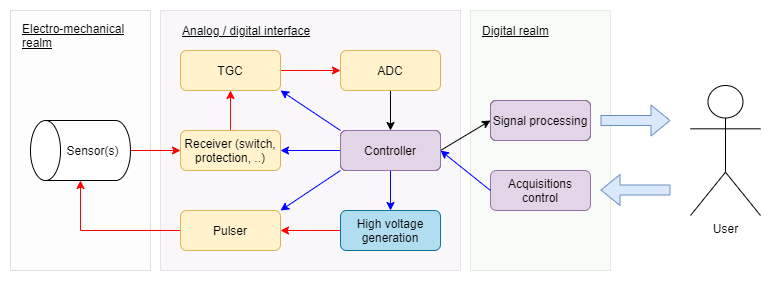
\includegraphics[width=\linewidth]{Fig1.png}
 \caption{Block diagram of a general ultrasound system. Analog components are in yellow, digital in purple, and high voltage in blue.}
 \label{fig:BlockDiagramme}
\end{figure}

The blocks consists in a Pulser, creating the initial energy transmission, a receiver to sort between the initial pulse and smaller subsequent signals, a Time Gain Compensation function to compensate for depth-related attenuation, and an ADC to digitize the signals. A controller needs to be coordination these different aspects in parallel, which is the reason for the choice of FPGAs over microcontrollers. Once digitized, the signal is exported to the user.

These blocks are used to create the pulse-echo pattern that ultimately creates an ultrasound image, be in in A-mode or B-mode. We will see that the analog elements, in yellow, can be integrated into single-chip devices.

As the sensors are mostly analog, and because of the low signals they yield, special care must be put on the analog parts (in yellow in \ref{fig:BlockDiagramme}) so that a satisfactory analog signal is extracted before digitization.




\subsection{State of the art and review of the ultrasound hardware designs}

\subsubsection{Design sources for the state of the art review}

A summary of the literature with respect to ultrasound system design, based on a review of components used, is presented in the table below. Most of these systems were design for academic research, and are not put to market. Both simple and high-end systems were considered in this review, as it is possible to exploit aspects of their design approach for use on simpler platforms. 

The objective of this review is not to design a single device, but to provide with an overview of the current state of art, and provide a benchmark for further specifications. The design of specific hardware, using only part of this review, would be a separate research topic.

% Please add the following required packages to your document preamble:
% \usepackage{booktabs}
 
\begin{table}[H]
\centering
\begin{tabular}{l|c|c|c|c|c|c}
\textbf{Reference}                               & \textbf{Elements} & \textbf{Voltage} & \textbf{Msps} & \textbf{Res} & \textbf{AFE-TGC}    & \textbf{Year}   \\ \hline
\cite{ahn_smartphone-based_2015}    & 16          & 70V     & 40   & 10   & AFE5808 & 2015 \\
\cite{assef_compact_2014}      & 128         & 100 Vpp & 50   & 12   & AFE5805 & 2014 \\
\cite{assef_design_2012}       & 128         & 100 Vpp & 50   & 12   & AFE5805 & 2012 \\
\cite{assef_flexible_2015}          & NA          & 100 Vpp & 40   & 12   & AFE5805 & 2015\\
\cite{batbayar_hardware_2018}     & 4x32        & NA      & 80   & 10   & NA      & 2018 \\
\cite{bharath_compact_2018}  & 8           & 105V    & 50   & 16   & AFE5809 & 2018 \\
\cite{bharath_novel_2016}     & 8           & +-50V   & 40   & 12   & AFE5808 & 2016 \\
\cite{bharath_portable_2015}      & NA          & NA      & NA   &      & NA      & 2015 \\
\cite{chang-hong_hu_design_2008}   & 1           & 15V     & 120  & 12   &         & 2008 \\
\cite{chatar_analysis_2016}        & 16          & NA      & 150  & 14   & NA      & 2016 \\
\cite{cheung_multi-channel_2012} & 128         & NA      & 80   & 10   & AD9272  & 2012 \\
\cite{dusa_low_2014}             & 8           & 100 Vpp & 65   & 12   & AFE5809 & 2014 \\
\cite{fritsch_full_nodate}          & 1           & 50-400V & 80   &      & NA      & NA \\
\cite{govindan_reconfigurable_2015} & 8           & NA      & 250  & 8    & VCA8500 & 2015 \\
\cite{hager_ultralight:_2017} & 64          & 100Vpp  & 32,5 & 12   & AFE5851 & 2017 \\
\cite{hewener_highly_2012}      & 128         & +-75V   & 80   &      & AD9273  & 2012 \\
 \cite{ibrahim_towards_2018}     & 64          & 12 V    & 20   & 12   & NA      & 2018 \\
 \cite{jonveaux_arduino-like_2017} & Single      & 100Vpp  & 22   & 9    & AD8331  & 2018 \\
 \cite{kim_smart-phone_2017}       & 128 (32 ch) & +-80 V  & 50   & 12   & NA      & 2017 \\
\cite{kruizinga_compressive_2017}  & Single      & 100 Vpp & 200  & 12   & NA      & 2017 \\
\cite{kushi_ultrasonic_2017}     & Single      & NA      & 100  & 14   & NA      & 2017 \\
\cite{lee_new_2014}             & 16          & NA      & 40   &      & AFE5808 & 2014 \\
\cite{li_new_2014}         & Single      & 80 V    & 40   & 12   & AD9276  & 2014 \\
\cite{matera_smart_2018}       & 8           & 6V      & 75   & 14   & AFE5809 & 2018 \\
\cite{nguyen_estimating_2019}    & 2           & 18V     & 40   & 10   &         & 2019 \\
\cite{pashaei_flexible_2020}      & 8           & 10V     & 80   & 12   & AD9276  & 2020 \\
 \cite{peyton_comparison_2018}     & 32          & NA      & 20   &      & Custom  & 2018 \\
\cite{qiu_delayed-excitation_2018} & Single      & +48V    & 160  &      & AD8331  & 2018 \\
\cite{qiu_ultrasound_2020}         & 1           & 60V     & 250  & 12   & TC6320  & 2020 \\
\cite{ricci_programmable_2006}   & 1           & 100 V   & 64   & 14   & MAX4107 & 2006 \\
\cite{roman_open-source_2018}   & 64          & +-50V   & 80   & 12   & AD9276  & 2018 \\
 \cite{vasudevan_programmable_2014} & Single      & 100 Vpp & 250  & 12   & VCA8500 & 2014 \\
\cite{wall_high-speed_2010}        & NA          & 12 V    & 65   &      & NA      & 2010 \\
\cite{weng_fpga-based_2015}      & 16          & 100V    & 150  & 10   & Max2077 & 2015 \\
\cite{zhang_high_2019}            & 64          & 100V    & 80   & 14   &         & 2019 \\
\cite{zhang_multi-channel_2017}     & 8           & 70V     & 250  & 16   & QT1138  & 2017    

\end{tabular} 
\caption{Review of ultrasound hardware designs, detailing speed of acquisitions (Msps), Resolution (Res.) and possibly the other supporting devices}
\label{tab:benchmarklite}
\end{table}


From these designs, as volumes are not specified, it may be possible to guess the cost of components, but searching for a comparative cost would not yield relevant information.

\subsubsection{High voltage pulser (transmit stage)}

There are several options to design a high voltage pulser, depending on the required specifications, such as size, power use, voltage range, or cost. A summary pf components is presented below.

%Discrete pulsers have been used. Design include dual stage designs, based on a driver ( MD1213 or MD1711) and high voltage FETs. Couples seen could be TC7320 and MD1810 \cite{kang_system--chip_2016}.
%Integrated alternatives are HV7361/HV7351 designs, HV748 being deprecated. Contrarily to the HV7361, the 8-channel HV7351 also allows for predetermined transmit patterns.

%Alternatively, for customised waveform pulser, a DAC and power amplifier combination can be used \cite{matera_smart_2018}. %

\begin{table}[h!]
\begin{tabular}{p{0.2\linewidth} | p{0.3\linewidth} | p{0.45\linewidth} }%{lllll}
\textbf{Typology}                    & \textbf{Components}          & \textbf{Examples} \\

Drivers and high voltage FETs  
& MD1213+MD1711, TC7320+MD1810 , EL7158+TC6320
& \cite{sharma_development_2015,wu_novel_2013,ching_chu_designing_nodate}                 \\

Integrated Chips 
& HV7361/HV7351, HV748, STHV800, LM96551
& \cite{martins_-scan_2017,zhang_multi-channel_2017,hewener_highly_2012,worthing_using_2016}                 \\

Multiplexers/switches 
& MAX14808
& \cite{rodriguez-olivares_improvement_2018,lee_new_2014,garcia_piezoelectric_2014,boni_ula-op_2016} \\

Signal generator and power amplifier 
& THS5651A+LT1210CS, TCA0372
& \cite{matera_smart_2018,choi_versatile_2020}
\end{tabular}
\caption{Pulsers, by approach}
\label{tab:pulser}
\end{table}

Contrarily to the HV7361, the 8-channel HV7351 also allows for predetermined transmit patterns.

\subsubsection{Switches}

Switches allow to select the element of interest, as well as possibly remove unwanted high voltage components. Transmit / receive (T/R) switches are used there, such as LM96530 \cite{vasudevan_programmable_2014}, the MAX14866 or the HV2605, HV2201, HV20220 \cite{li_new_2014} chips. Switches can be integrated at the pulser level \cite{worthing_using_2016, hidayat_determination_2020} or on the receiving path, with a LM96530 \cite{gwirc_desarrollo_2019, roman_open-source_2018}. 

More simply, clipping devices (MD0100 \cite{li_new_2014, sharma_development_2015}, MMBD4148/MMBD3004 \cite{ching_chu_designing_nodate}) allow clipping of the signal on the receive path to protect it.

\subsubsection{Time Gain Compensation (TGC) Amplifiers}

Choice of discrete elements as amplifiers is relatively limited, from the AD8331 family \cite{grasel_characterization_2017,lay_progress_2016,brunner_how_2002}, or low noise amplifiers. In order to dynamically adjust the gain, it is expected that the variable gain amplifier can be finely controlled as a function of time. The gain range would usually range between 0dB and 40dB to 80dB \cite{sharma_development_2015,levesque_architecture_2011}.  The AD8335 is a simpler amplifier with 80dB gain \cite{tortoli_ula-op:_2009}. AD604 \cite{yang_wearable_2019}, a dual variable amplifier with a gain of 48dB, was also considered.

\subsubsection{Analog to digital converters (ADCs)}

Once the signals amplified, it is relatively easier to match the ADC range and make a full use of its digitization range. As such, most of the designs present ADCs mostly ranging from 10 to 14 bits, and speeds from 40 to 150 Msps, depending on the sensors frequency. In simple design, mono-frequency sensors from 1MHz to 15MHz are used, sometimes with higher frequencies, though multi-frequencies \cite{sun_multi-frequency_2018} devices have also been developed \cite{lukacs_single-element_1998,foster_new_2009}. In some cases, FIFO buffers between the ADC and the controler were used \cite{yang_compressed_2009}, for example with the AL422B. 

\subsubsection{Electronic Analog Front-End (AFE)}

In more recent designs, ADCs and some or part of the analog components (in yellow in Fig 1) are often integrated in analog front-end chips, which allow for a simpler integrated design, albeit at the expense of making a design more expensive and less open. These components integrate the pulser, channels management, amplifier and digitization functions in a single chip. Different families were identified during this review. 

\begin{itemize}
\item \emph{AD927X} systems usually have 8 channels, with a 12-bit ADC from 10 MHz to 80 MHz, with time compensation amplifiers, widely used \cite{di_ianni_system-level_2016,hewener_highly_2012,  raj_programmable_2018, cheung_multi-channel_2012, alqasemi_fpga-based_2012, batbayar_hardware_2018,  techavipoo_ultrasound_2012}. 
\item The \emph{AFE58XX} family has 8- to 32-channel AFEs from 50-65MSPS, with LNA, VCAT, PGA, LPF, ADC, and possibly Continuous Wave (CW) Mixer \cite{assef_flexible_2015, assef_design_2012, assef_compact_2014, assef_initial_2016, bharath_fpga-based_2015, bharath_novel_2016, lee_new_2014, hager_lightprobe:_2017, bharath_compact_2018, kidav_architecture_2019}.
\item Finally, the \emph{MAX2082 and MAX2077} have 8 channels, including a high voltage pulser and transmit/receive switch (TR switch), but offer no digitization capability \cite{hewener_mobile_2019, weng_fpga-based_2015,seo_non-invasive_2018,sabbella_dhvani_2021}.

\end{itemize}

These AFEs all include several channels, which is not necessary for a single-element design. However, AFEs may still be useful in multi-channel designs in order to improve space and cost efficiency, and may prove useful in posterior design with improving controllers.

\subsubsection{A challenge: high-voltage generation}

High-voltage components were also reviewed, however, the topic of efficient high-voltage sources is not considered in most publications, apart from \cite{xiao_design_2013}. High-voltage design for ultrasound has been a particular point of interest. The ideal requirements for a good high-voltage design would involve developing a unit with a small footprint, low power consumption, and settable levels between 0 to 90V, ideally with another source for 0 to -90V for bipolar pulses, which would usually function with a current supply of 25-30mA.  Early designs \cite{brown_low-cost_2002} achieved 350V pulses with \$50\, but finding a working design is still a challenge today. In addition, only few researchers are sharing their designs \cite{tang_computerized_2014}, even considering existing detailed datasheets provided by manufacturers \cite{granata_designing_2020}. Devices such as the LM96550 were not considered in this review because of their relative important physical size. In the open-source literature, designs  used of an expensive RECOM device, providing a 0 - 120V range, or a NMT0572SC, providing 24, 48 and 72V rails, as well as the LT3494 with a rail up to 39V. Other alternatives were considered, namely the \emph{MAX668} (which operates from O to 150V), \emph{MAX1856} (between -80V and -24V), an \emph{MIC3172} design, using an \emph{HV9150} to reach up to 200V, or a \emph{MAX15031} of up to 80V. The \emph{DRV8662} family, including the DRV2700, also has been used to provide rails for up to 105V. Older devices were seen using integrated devices, such as the PICO 5SM250S DC-DC. 

In order to optimize power consumption, electrical impedance matching \cite{rathod_review_2019} has to be used to improve the level of energy transmitted to the transducer, especially with low-cost vector network analyzer (VNAs), like the 40\$ NanoVNA, usable in MHz-range transducers), which has allowed for some interesting developments \cite{garcia-rodriguez_low_2010, wei_design_2020} and can be used for improving the overall signal-to-noise ratio.


\subsubsection{Mechanical sweeping}

When designing any 2D ultrasound imager, a system capable of sweeping the space to be imaged is required. To minimize hardware costs, the space can be imaged by mechanically sweeping a single piezoelectric element across the target scene \cite{shaw_mechanical_1977,matzuk_novel_1978,wilkinson_principles_1981}, therefore requiring only a single channel of electronic hardware for data acquisition  \cite{saijo_development_nodate}. This sweeping principle has been used in several experimental setups, including \cite{chang_low-cost_2009}, and was used in older mechanical probes, which are based on either continuous rotation (Kretztechnik AR3 4/5B/A, ATL 724A, ... ) of the transducer to accommodate plane sweeping \cite{holm_new_1975}, sometimes with multiple transducers to allow for multiple images per rotation or with mechanical sweeps (Interspec Apogee, Diasonics probes, Kretztechnik AW14/5B/A, HP 21412A, ... ) \cite{jonveaux_review_2019}. This approach was initially more commonly seen in intra-cavity probes, due to space constraints \cite{hisanaga_high_1980}. 

For cardiac scans of small animals, heartbeat and target size require in excess of 100 frames per second (fps) with a spatial resolution of 100um or less:  \cite{lei_high-frame_nodate} implemented for example a 30-50 MHz real-time ultrasound single-element device that scans at 130 fps. Higher frequencies imaging transducers are  relatively smaller in size, which makes them ideal candidates for mechanical sweeping when arrays are too large. However, this implies strong positioning control and precision motors, requiring, for example, optical encoder and  piezoelectric motors \cite{carotenuto_very_2004}, with a requirement of injecting as little noise as possible on the analog processing path. Other uses of piezoelectric actuators include the use of bimorphs \cite{bezanson_low-cost_2011}, reaching 130fps for electromagnetic motors. Still, the weight borne by the actuator has to be limited \cite{brown_low_2013, huang_novel_2015}, a constraint also satisfied by MEMs \cite{choi_versatile_2020}. Alternatively, the use of mobile acoustic mirrors with fixed transducers was considered \cite{havlice_medical_1979}.

In laboratory designs where real-time imaging is not required, XYZ positioning systems with 3D-printed components have been used \cite{svilainis_electronics_2014, wang_high_2019, xu_enabling_2019}. \cite{bottenus_feasibility_2016}, for example, demonstrated that a three-axis translation stage allowed for precise position and orientation control of the transducer. 1-D systems, for example based on a transducer on a linear motor stage, can also be used  \cite{qiu_programmable_2011,govindan_reconfigurable_2015, soto-cajiga_fpga-based_2012,govindan_performance_2013}, which allows the system's transducer to sweep across the target scene. \cite{smith_design_2015} also uses a single transducer element in combination with a lower noise voice coil motor as the mechanical actuator, a compromise with significant estimated production cost savings (over 95\%), while keeping a relatively noise-free signal. 

Alternative displacements methods can be used, for example, using accelerometers to determine the position of the transducer  \cite{sobhani_portable_2016} or allowing for precise image reconstruction with an Arduino and Raspberry Pi setup \cite{herickhoff_low-cost_2019}, which can also be used in ultrasound training simulators \cite{farsoni_low-cost_2017}. In the case of skin imaging, another example is to use optical trackers like those used in computer mice \cite{zhang_free-hand_2019, poulsen_optical_2005, herickhoff_low-cost_2018}.


\subsubsection{Considerations when choosing acoustic  materials}

In most mechanical designs, an acoustic window, made of a material transparent to acoustic waves, is needed to seal the scanner mobile head from the external medium while minimizing signal loss. The first mechanical scanners used water-baths as an intermediate between the transducers and the subject \cite{schueler_fundamentals_1984}. A material regularly used for this is polymethylpentene (TPX), which can be used for example on high-frequency ultrasound scanners \cite{erickson_hand-held_2001,brown_low_2013}, or perspex \cite{bow_rotating_1979}.  Alternatively, \cite{qiu_ultrasound_2020} uses an acoustic window made from polydimethylsiloxane (PDMS, such as the silicon Sylgard 184) to minimize reflection and
attenuation during the ultrasound transmission, which can be used for reference targets \cite{lorenzo_experimental_2009,melde_holograms_2016}. 

More common materials can also be used. For example, polyimide can be used in ultrasound phantoms (reference imaging targets) \cite{xu_high-frequency_2008, lei_sun_high-frame_2008}, as well as sealant silicones \cite{lorenzo_experimental_2009} that mimic soft tissues. Polyvinyl alcohol or polyurethane, in addition to polyvinylidene fluoride (PVDF), have been be considered \cite{sikdar_novel_2014}  for device-patient acoustic coupling. Agar and gelatin are used on temporary phantoms \cite{vogt_development_2005,chun_ultrasound_2015}, where graphite powder reproduces tissue scattering, with no concrete application for the design of devices per se. 

\subsubsection{Controlers are piggy-backing on the development of open source FPGAs}

The controller, seen in Fig 1 as having a central function in ultrasound devices, has traditionally be a microcontroller, which had limitations not always compatible with ultrasound chips coordination as this happens fast, with several parallel communication taking place at the same time. A solution to was to use Direct Memory Access (DMA) optimized microcontroller designs \cite{kidav_architecture_2019}. However, thanks to the increasing accessibility of field-programmable gate arrays (FPGAs), digital signal processors (DSP), and systems-on-chip (SoC) for radio frequency signals processing is a strategic option. Along with the development of integrated AFE, they have accelerated the creation and availability of high-end programmable research platforms  \cite{roman_open-source_2018}.  In some designs, an additional micro-controller is set up between the FPGA and a USB bus \cite{pashaei_live_2018, schneider_fully_2010}, which can provide the FPGA with a configuration on the fly, and allowing access to the computation platform to set up the pulse-echo sequence parameters \cite{raj_microcontroller_2017, raj_8051_2016}, using in particular the Cypress families, either in USB 2 \cite{hu_design_2011,richard_low-cost_2008} or USB 3 \cite{lewandowski_low-cost_2012,qiu_delayed-excitation_2018,qiu_ultrasound_2020,ahn_smartphone-based_2015}, but also through Ethernet as well (eg with a CP2200) or WiFi.

FPGAs improve the potential for developing ultrasound imaging systems with small form factors and creating high-performance devices with reduced power consumption \cite{dusa_low_2014}. Configurable hardware makes the system resilient to future changes: designs can be adjusted without reprinting the circuit board \cite{zhang_fpga_2012, qiu_programmable_2010, ibrahim_single-fpga_2017}. From an open-source perspective, FPGA use has been supported by the development of new open-source toolchains \cite{shah_yosys+nextpnr:_2019}, thus opening a key technology to a wider public \cite{saiz-vela_low-cost_2020}.

FPGA allow more flexible connection between systems \cite{gilliland_architecture_2016,govindan_hwsw_2013}. Many high-end designs are based on peripheral component interconnect express (PCIe) due to high bandwidth requirements \cite{zimmermann_high_2018, lewandowski_low-cost_2012, kidav_architecture_2019}, but the complexity of PCIe is an obstacle to low-cost designs. In \cite{luc_jonveaux_un0rick_2019}, the Raspberry Pi's 40-pin header was used as a simple, standardized interface for developing extension boards. 

\subsubsection{Transmission of the digital information - bandwidth reduction}

Most microcontrollers lack sufficient bandwidth to digitize and process the full ultrasound signal at radio frequencies. Therefore, microcontroller-based systems typically use a pre-processing channel, possibly including a envelope detector in hardware prior to digitization of the signal, so that the signal bandwidth is reduced to that of the amplitude-modulating information. However, envelope detectors in hardware typically have a fixed cutoff frequency, which prevents them from being adaptable to different transducer frequencies.

Another possible technique is the use of quadrature sampling to preserve both amplitude and phase information, combined with frequency downconversion to reduce the bandwidth requirement for data transmission, storage, and processing to that of the ultrasound modulation bandwidth, which can be significantly narrower than the maximum frequency of the signal \cite{peyton_comparison_2018}. Because frequency downconversion and quadrature sampling are used in software defined radios (SDRs) \cite{hager_design_2019, hager_lightprobe:_2019} to capture the modulated information on a radio frequency (RF) carrier, SDR hardware can serve as a drop-in replacement for quadrature sampling hardware, as in the "rtl-ultrasound" open-source project \cite{meng_rtl-ultrasound_2019}.  As such, demodulation techniques would allow shifting signals from higher frequencies to lower, allowing slower acquisition techniques and leaner hardware. 




\newpage

\section{Signal processing steps}

\subsection{Conventional signal processing considerations}

In parallel to the hardware analog part, the digital component of acquisition systems is used, through its intrinsic flexibility, to provide a platform of choice to implement digital processing techniques. Now that we have covered the hardware aspects of the research, we now aim to provide the reader with resources describing an basic components of the signal processing path, i.e., signal filtering, envelope detection, signal compression and scan conversion \cite{basoglu_computing_1998}, and in a second time review more recent considerations.

\begin{figure}[H]
 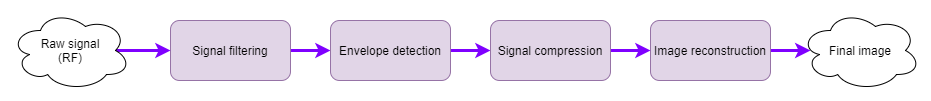
\includegraphics[width=\linewidth]{Fig2.png}
 \caption{Block diagram the signal processing path}
 \label{fig:SigProc}
\end{figure}

The signal processing step has one goal, that is to extract the right information from the raw electrical signal into an actionable information for the user. 

Upstream, \textbf{\textit{general filtering}} has been commonly used early in the processing pipeline, often close to the ADC via DSPs and FPGAs, to remove unwanted noise from RF signals while preserving the bandwidth of interest \cite{assef_modeling_2019, levesque_real-time_2009}, so to ensure a clean signal for further processing.

Once the signal is cleaned, it is possible to extract the information from the radio-frequency signal, which is provided by the \textbf{\textit{envelope detection}} step. Is transforms the RF signal into a human-readable image, for example using a Hilbert transform. Different envelope-detection methods and algorithms have been explored in DSPs and FPGAs \cite{chang_novel_2007, assef_fpga_2019, assef_modeling_2018}.

At this stage, and for B-Mode imaging, \textbf{\textit{deconvolution}} can be used to remove the usual blur of a single point image, due to the transducer geometry. The size of the blur in relation to the actual dimension of the point source is a measure of the resolution of the system. To record this behaviour, a point-spread function ) is measured, i.e., the "impulse response" of the system.  Knowing a system’s PSF makes improving the image resolution an inverse problem  \cite{jensen_deconvolution_1993,dalitz_point_2015}, and establishes the possibility of recursively reconstructing the true position and shape of the point through deconvolution \cite{dalitz_point_2015}.  

Once the image is assembled, \textbf{\textit{Amplitude compression}} can be used to further reduce  transfer rates needs between hardware and software, which are often a bottleneck. In this sense, having upstream compression would alleviate these bottlenecks \cite{soto-cajiga_fpga-based_2012, akkala_fpga_2014}. Alternatives \cite{akkala_compression_2014, boonleelakul_compression_2013} include  adjusting high electronics dynamic ranges (12 bits and more) to the 8 bits of LCDs and CRTs, for example using the ITU-T G.711 standard (or the a-law) used in sound compression.

\textbf{\textit{Image reconstruction}} is the last step to reconstruct a human-readable images. In the case of mechanical sweeping of an imaging area or volume, the scanned data may not correspond to a Cartesian grid, so a coordinate mapping step, called scan conversion, is often necessary before displaying the captured image.
Several algorithms have been developed to tackle this issue \cite{ophir_digital_1979}, with a focus on real-time requirements \cite{csany_real-time_2019}.

\subsection{Recent signal processing considerations}



It can be noted that element sensors (often focused as a given depth) have good characteristics to image around this region of depth. However, outside of this fixed depth, the resolution quickly degrades - which can can be alleviated by using \textbf{\textit{Synthetic Aperture Focusing (SAF)}}  \cite{andresen_synthetic_2011, assef_flexible_2015, li_initial_2018, lewandowski_low-cost_2012, zhang_synthetic_2016}. Other synthetic aperture techniques have been widely discussed, for example in \cite{gunarathne_strategies_2013, jeon_novel_2019} or earlier on \cite{burckhardt_experimental_1974}. Similarly, Monostatic Synthetic Aperture Scanner and Monostatic Fixed Focus Scanner are approaches worth citing in the review of data processing, as developed by \cite{bottenus_implementation_2015, ylitalo_ultrasound_1994,heuvel_development_2017, nikolov_fast_2008}, aiming at improving images quality.  

At the pulser stage, one can use \textbf{\textit{barker codes}}  \cite{zhang_evaluation_2019,wang_research_2021} to  improve image resolution by shaping the excitation signal itself \cite{isla_coded_2017}. It has been shown for example that it is possible to improve lateral as well as axial resolution  \cite{fujita_effect_2017, chun_ultrasound_2015, kim_real-time_2018}.

A more complex approach on the signal shaping and receiving is \textbf{\textit{compressed sensing (CS)}} : traditional 2-D and 3D ultrasound require the use of complex sensors, with matching hardware such as cabling. There are available, still costly - but such sensors require more hardware and become ultimately more complex and expensive to produce. 
It appears that classical sampling is challenged by the signal processing "compressed sensing" field \cite{liutkus_imaging_2014,hua_compressed_2011}. This allows for reconstruction of a signal with fewer samples than dictated by the Nyquist-Shannon sampling theorem. Starting with time reversal applications \cite{montaldo_time_2004, montaldo_building_2005} or \cite{sarvazyan_comparative_2009}, compressing measurements before sensing enable new ultrasound applications, where positioning a plastic coding mask in front of the aperture \cite{fedjajevs_ultrasound_2016} or simply for the purpose of envelope extraction \cite{kim_signal-processing_2020}.  One can therefore encode individual volume pixels or voxels using a 'chaotic' medium  \cite{luong_compact_2016}, allowing 3D imaging using a single-element ultrasound sensor and opening doors to simpler hardware and again new applications \cite{kruizinga_compressive_2017}. Different works have been dedicated to creating the phase encoding masks \cite{van_der_meulen_spatial_2017} or even using random interference to improve image resolution \cite{ni_high-resolution_2020}.


From a transverse perspective, \textbf{\textit{machine learning}} (ML) has shown promising improvement in terms of both image quality improvement \cite{wang_high-resolution_2019, hewener_mobile_2019} and support for image interpretation \cite{divya_krishna_computer_2016}, even in A-mode \cite{brausch_classifying_2019}. An open-source MT tool to interpret Doppler signals \cite{dhutia_open-source_2017} has also been developed. ML also applies to texture imaging, as earlier proposed by reviewing "Average Higuchi Dimension of RF Time series" \cite{moradi_detection_2006}, or in to-non imaging techniques, such as mixing monitoring \cite{bowler_monitoring_2020}.


\newpage
\section{Conclusion}

A review of state-of-the-art ultrasound hardware designs and implementation was presented in this article, opening on new challenges and considerations as ultrasound technologies are maturing and new approaches are made possible.

Though there was a lack of available open hardware on the market, there seems to be sufficient information available to assemble a proof-of-concept system that offers a safe, cheap and portable alternative to other imaging technologies, as demonstrated by the un0rick and lit3rick designs. More sophisticated systems will surely emerge from open designs, building on recent components and new controllers.

The number of more complex channel designs appears to have grown due to the increased availability of electronic components and AFE integration of additional analog channels, these systems also have improved functionality. However, these designs also require rapid logic control, which is today not easily possible from an open-source perspective. In addition, compressed sensing allows for drastic improvements in image quality while reducing the number of sensors and the corresponding hardware required. 

From an academic perspective, there is significant evidence in the literature demonstrating the utility of open-source design, both from a medical perspective but also for private and public research purposes, not to mention education. Researchers have identified ultrasound as a safe, low-cost solution in medically under-served regions and markets with rising health costs. There is also increased interest in terms of private-sector research and development, as indicated by the abundance of recent works and new projects indicating the innovative aspects of the topic. 

Open-source hardware has a potential to change the shape of ultrasound research, by having replicable systems possibly customized to specific applications, addressing both niche needs and accessible, lower-end requirements.


%Joining forces with industrial players such as low cost manufacturers in Shenzen, along with quality experts and medical staff to build fully open-source devices is clearly something that could be possible for the production of veterinary, research, or NDT devices.

In general, open source ultrasound hardware research \cite{roman_open-source_2019} is accelerating, and it is our hope that this article will encourage other researchers, manufacturers \cite{yu_direct_2020} and makers to share their work. 

\section*{Acknowledgment}

The main author would like to thank the co-authors for their contributions and express appreciation to the Open Ultrasound Society for their insights and exchanges on \href{https://join.slack.com/t/usdevkit/shared_invite/zt-2g501obl-z53YHyGOOMZjeCXuXzjZow}{Slack}. Special thanks to David, Vladimir, Andrew, Bogdan, and Ahmed.

\clearpage

\section*{Supplementary information}

Equipment providers include:
\begin{itemize}

\item Avtech \cite{qiu_high-resolution_2020,lei_high-frame_nodate},
\item Biosono \cite{biosono_sonolab_nodate,bharath_fpga-based_2015},
\item Eurosonic \cite{jin_optimization_2017, mostavi_application_2017, ranachowski_mechanical_2020, vadalma_smartphone_2020}, 
\item Lecoeur Electronique \cite{lecoeur_bluetooth_nodate, tortoli_ula-op:_2009, zhang_toward_2018, al-aufi_thin_2019},
\item MKC \cite{park_ultrasound_2019},
\item Olympus \cite{veenstra_generating_nodate,choi_versatile_2020,chun_ultrasound_2015,xu_low-cost_2007},
\item Optel \cite{ scholle_pulse_2018, ratajski_application_2017, nowak_evaluation_2020, karjalainen_multi-site_2012},
\item Osun \cite{vadalma_smartphone_2020,bharath_fpga-based_2015}, 
\item Ultratek \cite{veenstra_generating_nodate, perez-sanchez_numerical_2020, chen_ultrasound_2016, wang_preliminary_2019}
\item
Verasonics \cite{peyton_front-end_2017, george_portable_2018, kang_new_2017, hager_ultralight:_2017} 
\item or  the Fraunhofer Institute \cite{zimmermann_highly_2019, zimmermann_miniaturized_2018, zimmermann_high_2018} 
\end{itemize}

Other suppliers have made smaller contributions to the literature \cite{ozdemir_remote_2018}, such as Socomate \cite{gil-alba_morphological_2019}, MATEC TB-1000 \cite{kielczynski_thermophysical_2017} JSR Ultrasonics \cite{cramer_ultrasonic_2015}, or high-speed Dr Hillger's USPC \cite{hillger_high_2016}. 

\clearpage

\bibliographystyle{apalike}

\bibliography{all,new,LIGHT}  

\end{document}

